% SPI Handler

\textbf{Top design - PSoC Creator 3.0}

Topdesignet (figur\ref{lab:topdesign_spi}( består af en SPI blok, samt 3 digitale output pins. Herunder beskrives hvordan elementerne i topdesignet skal indstilles.

\begin{figure}[H] \centering
{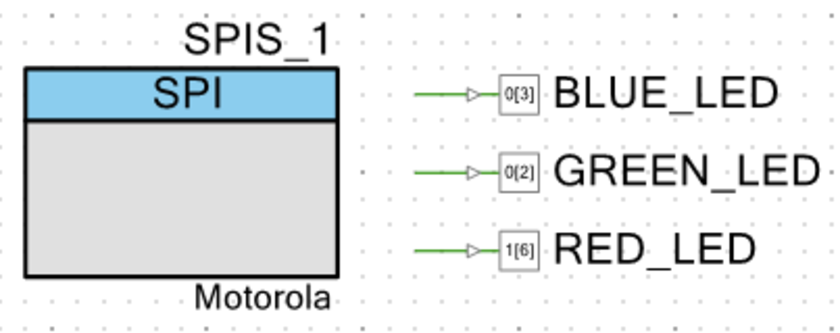
\includegraphics[width=\textwidth]{filer/implementering/spi/spi_handler_topdesign}}
\caption{Topdesign for SPI og led}
\label{lab:topdesign_spi}
\raggedright
\end{figure}

Basis indstillingerne for SPI blokken ses i figur \ref{lab:spi_basic_config}. Mode sættes til slave, og SCLK mode sættes til CPOL=0, CPHA=0.

\begin{figure}[H] \centering
{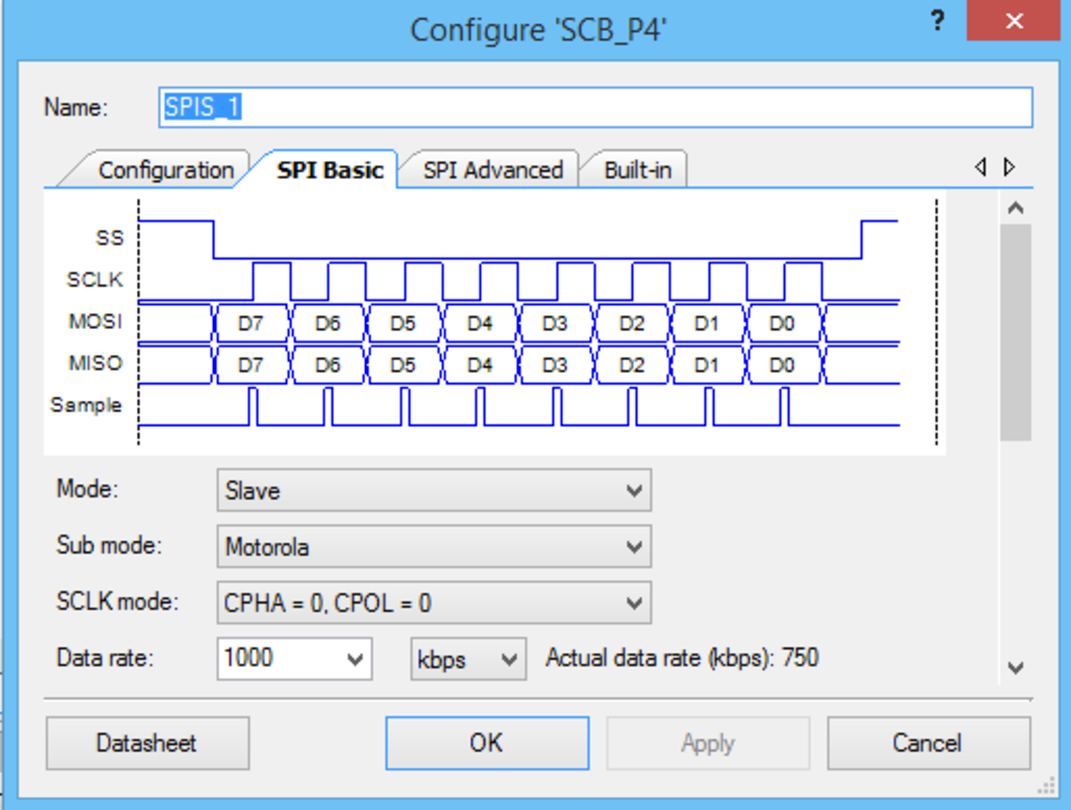
\includegraphics[width=\textwidth]{filer/implementering/spi/spi_handler_topdesign_spi_basic}}
\caption{Konfigurering af SPI (SPI basic)}
\label{lab:spi_basic_config}
\raggedright
\end{figure}

De avancerede indstillinger for SPI blokken ses i figur \ref{lab:spi_advanced_config}. Buffer size sættes til 8 bit for både RX og TX. Interruptet sættes til internt og interrupt kilden er RX FIFO not empty og RX FIFO full.
\begin{figure}[H] \centering
{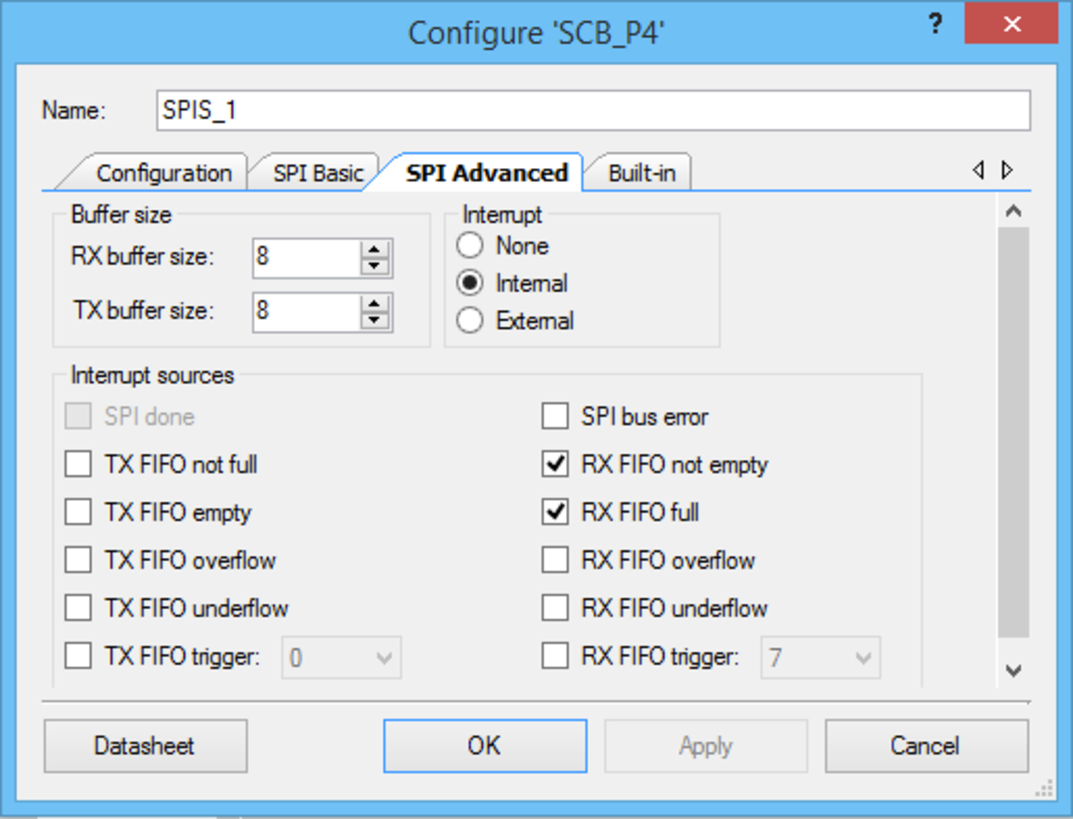
\includegraphics[width=\textwidth]{filer/implementering/spi/spi_handler_topdesign_spi_advanced}}
\caption{Konfigurering af SPI (SPI advanced)}
\label{lab:spi_advanced_config}
\raggedright
\end{figure}



De 3 output pins (GREEN\_LED, BLUE\_LED, RED\_LED) skal sættes til digital output uden hardware connection.
Figur \ref{lab:led_pins_config} viser hvordan indstillingen skal være, dette er gældende for alle 3 pins. 

\begin{figure}[H] \centering
{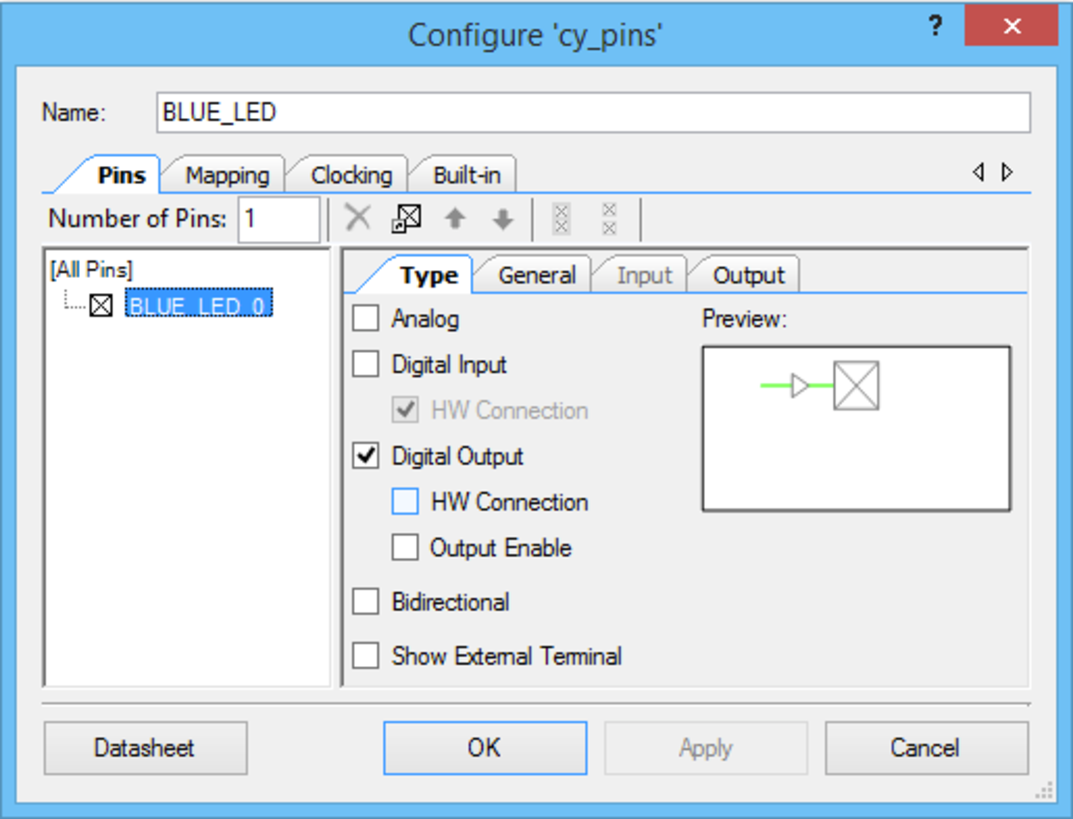
\includegraphics[width=\textwidth]{filer/implementering/spi/spi_handler_topdesign_led}}
\caption{Konfigurering af pins}
\label{lab:led_pins_config}
\raggedright
\end{figure}



\textbf{ISR}

\begin{lstlisting}[language=C]

CY_ISR(isr_spi_rx)
{
	Save recived char in cmd
	Save cmd in spiBuffer[spiCounter]
	Increment spiCounter

if ((cmd == 'R') || (cmd == 'C') || (cmd == 'L')){
    	switch (spiBuffer[0]) {
    		case 'A':
			Turn on RGB led green
			Clear tx-buffer 
			Reset spiCounter 
			Call method:                
		case 'D':
			Turn on RGB led red
			Clear tx-buffer 
			Reset spiCounter 
			Call method:  
		case 'P':
			Disable interrupt			
			Save data for humidity and temperature             
            Call method: config(humiValue, tempValue)
            Clear tx-buffer 
			Reset spiCounter 
            Re-enable interrupt  
		case 'V':
        		Turn on RGB led red
			Clear tx-buffer   
			Write UnitNo  to tx-data		
			Reset spiCounter 
			Call method:  
       	case 'L':
        		??
        		Call method: 
       	case 'R':
			??
			??
      	case 'C':
           	Clear tx-buffer   
           	Reset spiCounter 
    	}
\end{lstlisting}